\section{Test di circuiti digitali}\label{capitolo1}
Quando si vuole realizzare un nuovo prodotto hardware come uno smartphone o semplicemente anche un nuovo modulo wifi si parte sempre dalle richieste del cliente e da queste si passa alla stesura di un documento di \emph{specifica}, alla \emph{progettazione} del sistema ed infine alla \emph{verifica} che il sistema progettato è conforme alla specifica. Dopo queste fasi iniziali però si deve tradurre il progetto in uno hardware che si possa costruire in modo semplice ed efficiente. Il passo finale prima di poter commercializzare il prodotto è quello del collaudo in quanto, in molti casi possono sorgere problemi di fabbricazione e, pur essendo il progetto corretto il sistema finale non funzionerà. Lo scopo di questo capitolo allora è quello di capire quali sono le tecniche migliori per far collaudare un nuovo sistema. Primo fra tutti è quello di pensare al collaudo durante la fase di progettazione e prevedere un modo per rendere facile i test dopo aver prodotto il sistema.
Il modo più semplice per testare un circuito è quello di prelevare il componente terminato e inserire una serie di valori in ingresso e comparare i valori all'uscita per verificare che il risultato sia corretto come mostrato in \figurename\,\ref{fig:testbasic}.\\
\begin{figure}[b]
\centering
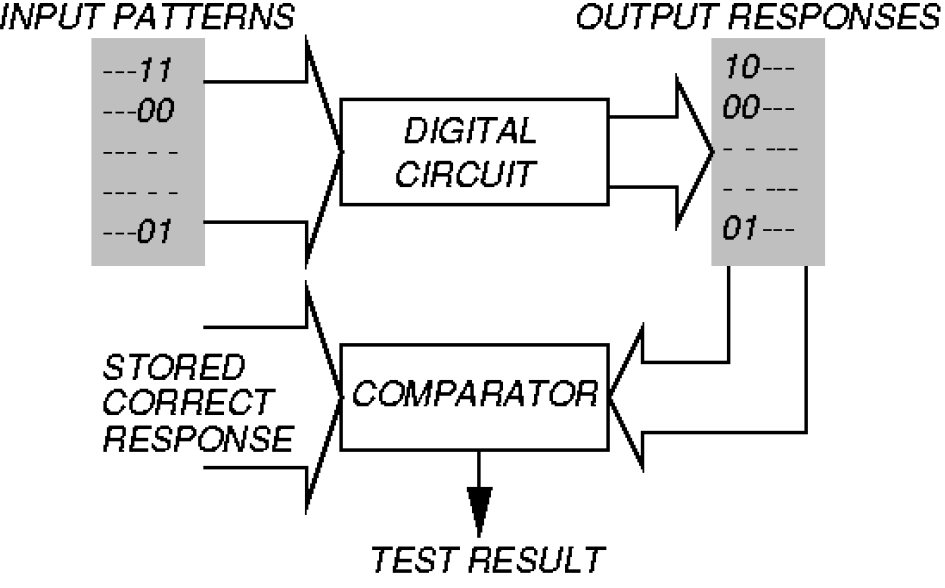
\includegraphics[scale=0.35]{img/testbase.png}
\caption{Collaudo di un sistema hardware}\label{fig:testbasic}
\end{figure}
Questo meccanismo può essere applicato a qualsiasi componente del circuito ma questa tecnica presenta diversi problemi, prima tra tutte il costo delle apparecchiature necessarie per l'esecuzione dei test; ad esempio per un ATE a 1024 pin che lavora ad una frequenza che varia tra \emph{0.5} e \emph{1 GHz} il costo è dato dal costo base più un certo costo per ogni pin.
$$\$1.2M + 1024 \times\$3000 = \$4,27M$$
Per tale apparecchiatura si dovrà inoltre prevedere un costo dovuto all'ammortamento, alla manutenzione e alla sua operatività che per il nostro esempio possiamo quantificare come:
$$
\begin{array}{cl}
= & Ammortamento + Manutenzione + Operativita \\
= & \$ 0.854M + \$ 0.085M + \$ 0.5M \\
= & \$ 1.439M/anno
\end{array}
$$
Tale costo si riflette sul prodotto finale, infatti, supponendo che la macchina lavori 24/7 avvremmo che il costo al secondo della macchina è pari a:
$$
\begin{array}{cl}
= & \$ 1.439M/(365 \times 24 \times 3600)\\
= 4.5 cent/sec
\end{array}
$$
Questo significa che ogni secondo di test costa \emph{4.5 cent} per questo motivo è necessario che il test dia risultati chiari ma che venga svolto nel minor tempo possibile.\\
Un altro problema che si può presentare è la granularità con la quale si effettuano i test, infatti più il livello al quale si effettua il test è basso meno costoso sarà la riparazione, ad esempio se il livello al quale si scopre il guasto è a livello di transistor il costo della sostituzione del transistor è quantificabile a \emph{1}, se il guasto viene individuato quando il transistor è montato su di una board allora il costo sale a \emph{10} se tale board è montata nel sistema prima di scoprire il guasto allora il costo di quel guasto sale a \emph{100} e così via; mano a mano che si sale di livello il costo di un guasto in termini di individuazione e riparazione diventa dieci volte più grande. Per questo motivo quando si effettuano i test le probabilità di individuare un componente difettoso devono essere le più alte possibili anche a costo di scartare qualche componente che non sia difettoso come mostrato in \figurename\,\ref{fig:probguasto}.\\
\begin{figure}
\centering
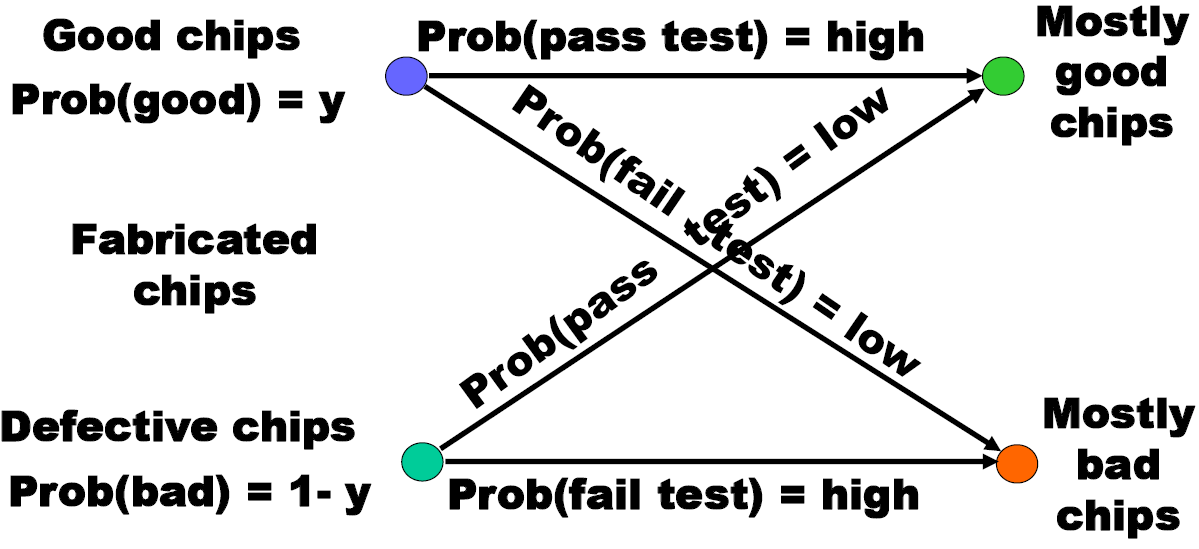
\includegraphics[scale=0.35]{img/probguasto.png}
\caption{Probabilità di individuazione di componenti guasti}\label{fig:probguasto}
\end{figure}
\subsection{I modelli di guasto}
L'individuazione dei difetti di fabbricazione è diventata perciò una parte fondamentale della fase di realizzazione di un sistema hardware, e come tale si è evoluta nel tempo passando da considerare i \emph{difetti di fabbricazione} come eventi sfortunati, a considerarli successivamente dei \emph{guasti} fino ad arrivare ai \emph{modelli di guasto} che si prefiggono lo scopo di creare un modello per ogni livello di astrazione per individuare i punti cruciali del circuito nel quale effettuare i test.\\
I guasti possono essere di diverso tipo e dovuti a diversi fattori, essi possono essere:
\begin{itemize}
\item Difetti di processo:
\begin{itemize}
\item Contatti mancanti
\item Capacità parassite
\item Ossidazione dei contatti
\end{itemize}
\item Difetti materiali:
\begin{itemize}
\item Difetti di carico (rotture o imperfezione nei cristalli)
\item Impurità sulle superfici
\end{itemize}
\item Guasti dipendenti dal tempo:
\begin{itemize}
\item Rotture elettriche
\item Elettromigrazione
\end{itemize}
\item Guasti da imballaggio
\end{itemize}
In \figurename\,\ref{fig:tabguasti} sono mostrati i principali guasti che si presentano su una PCB con le rispettive percentuali.\\
\begin{figure}
\centering
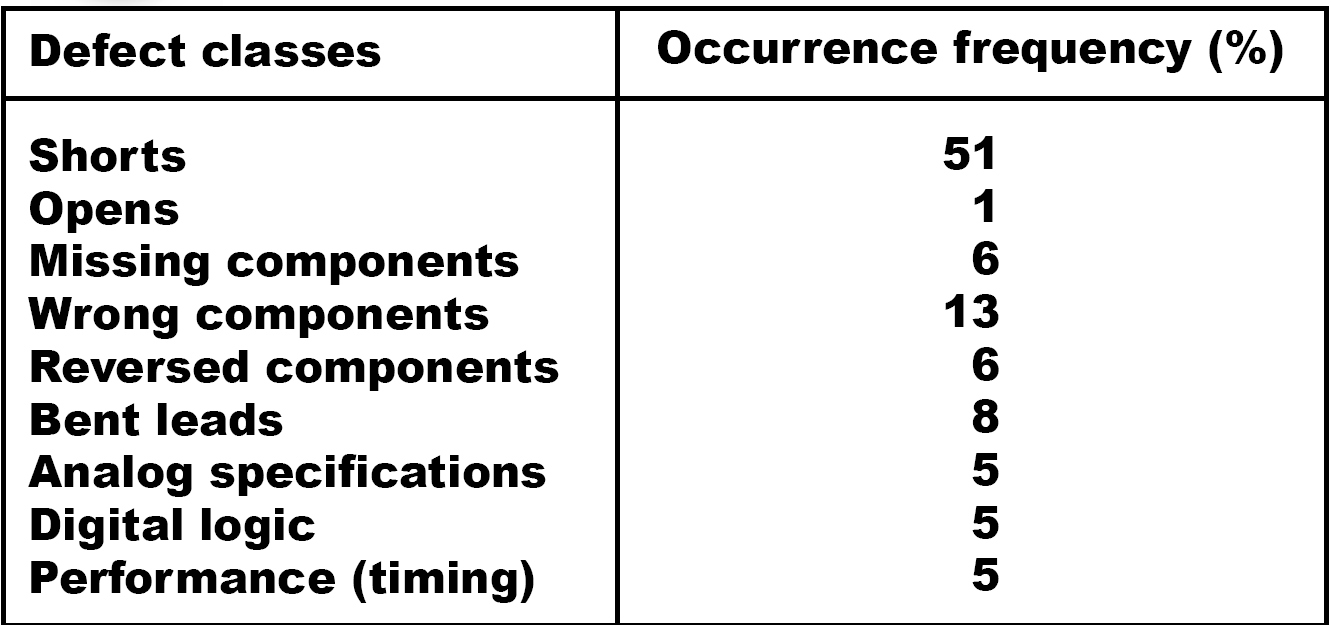
\includegraphics[scale=0.3]{img/tabguasti.png}
\caption{Percentuale dei guasti ad una PCB}\label{fig:tabguasti}
\end{figure}
Esistono diversi modelli di guasto i più comuni ed utilizzati sono:
\begin{itemize}
\item Single stuck-at faults
\item Transistor open and short faults
\item Memory faults
\item PLA faults
\item Functional faults
\item Delay faults
\item Analog faults
\end{itemize}
\subsubsection{Single Stuck-at fault}
Il primo modello che analizziamo è il \emph{Single stuck-at} in questo tipo di modello si assume che una linea del circuito rimanga bloccata ad un livello sia esso alto o basso. Il \emph{single stuck-at} ha tre caratteristiche che lo contraddistinguono, la prima è che solamente una linea si guasta, la seconda è che la linea guasta si blocca permanentemente ad un valore \emph{0} o \emph{1}, ed infine, la linea che si blocca può essere sia all'ingresso che all'uscita di una porta. Un esempio di circuito  XOR analizzato con modello di guasto a \emph{single stuck-at} è mostrato in \figurename\,\ref{fig:xorsinglestuck} dove sono indicati con un pallino verde i 12 punti di guasto mentre i possibili guasti sono 24 (due valori per ogni punto).
\begin{figure}
\centering
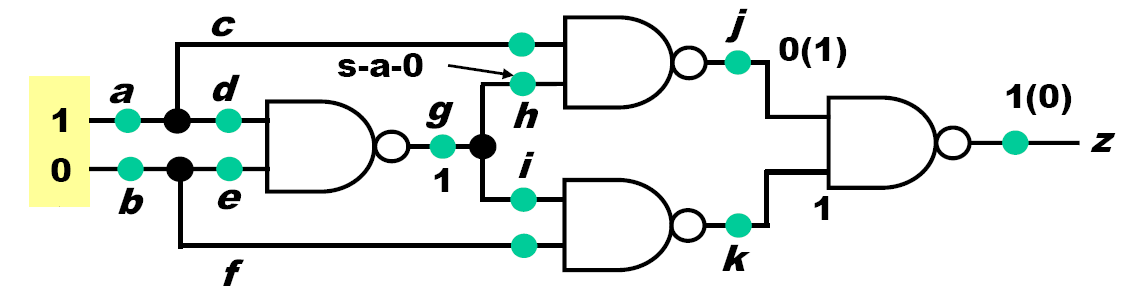
\includegraphics[scale=0.4]{img/xorsinglestuck.png}
\caption{Esempio di modello di guasto \emph{single stuck-at}}\label{fig:xorsinglestuck}
\end{figure}
Questo modello seppur semplice è supportato dall'evidenza empirica infatti è semplice da usare, può individuare anche altri tipi di guasti ed inoltre si presta ad essere modellizzato.\\
Questo modello può essere ampliato tramite la nozione di \emph{equivalenza di guasto} e quella di \emph{collasso dei guasti}. Si ha un'\emph{equivalenza tra guasti} quando due guasti $f_1$ e $f_2$ se tutti i test che individuano il guasto $f_1$ individuano anche il guasto $f_2$, se due guasti sono equivalenti le loro funzioni di guasto sono \emph{identiche}. Il \emph{collasso di guasti} si ha quando un circuito logico può essere diviso in un sottoinsieme equivalente dove tutti i guasti del sottoinsieme sono equivalenti, il collasso dei guasti avviene prelevando un guasto da ogni sottoinsieme.
In \figurename\,\ref{fig:equivaport} sono mostrate le regole di equivalenza per le diverse porte logiche.\\
\begin{figure}
\centering
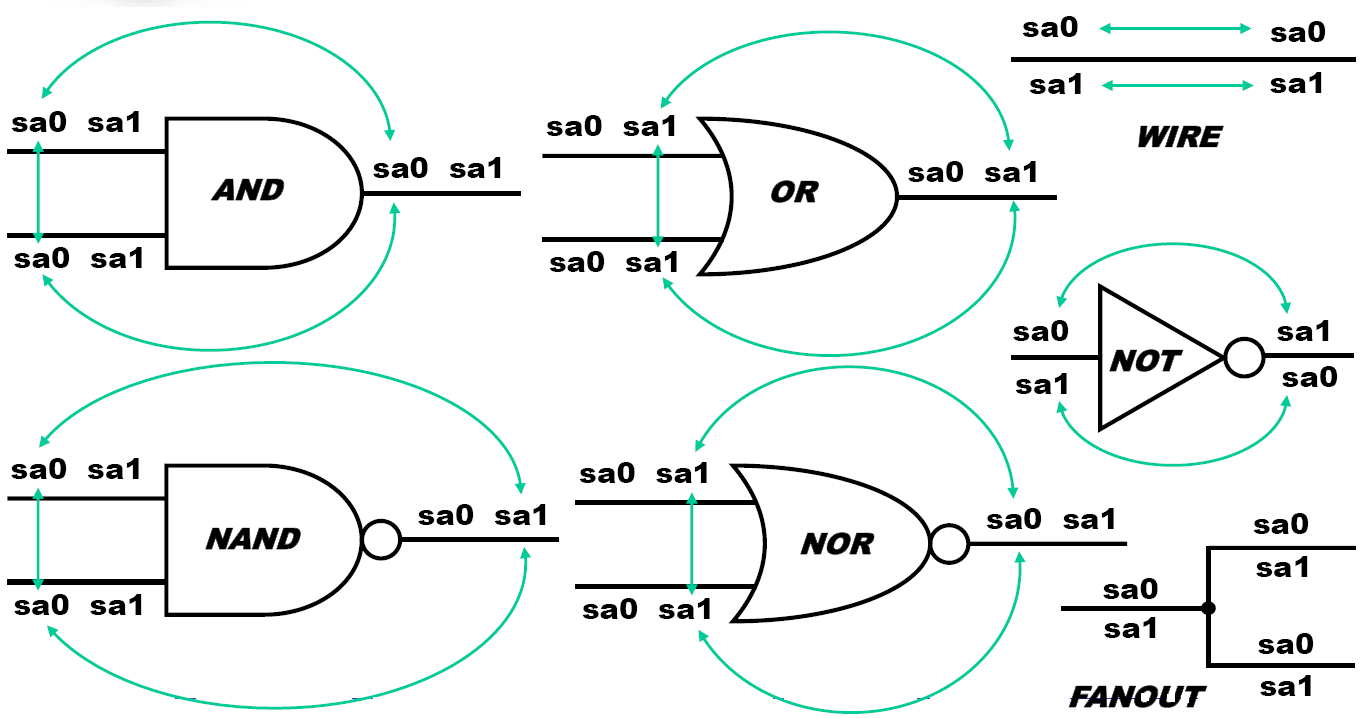
\includegraphics[scale=0.3]{img/equivaport.png}
\caption{Equivalenze tra le diverse porte logiche}\label{fig:equivaport}
\end{figure}
Un altro concetto che vogliamo introdurre è quello della \emph{dominanza} tra guasti, se tutti i test che individuano $f_1$ individuano anche un secondo guasto $f_2$ allora si dice che $f_2$ domina $f_1$.\\
Gli ingressi primari e i bracci dei \emph{fanout} di un circuito combinatorio sono chiamati \emph{checkpoints}; un teorema afferma che se un insieme di test individua i guasti su tutti i checkpoint di un circuito combinatorio allora quello stesso insieme di test individua tutti i guasti del circuito.\\
Il modello a \emph{multiple stuck-at} prevede, rispetto al modello a singolo stuck-at, che più linee contemporaneamente possano essere bloccate in una determinata combinazione di guasto. Il numero totale di combinazioni di guasti in un circuito con \emph{k} punti di guasto è di $3^k-1$.
\subsubsection{Transistor faults}
Esistono diversi modelli di guasto che riguardano i transistor che fanno riferimento a dei comportamenti anomali di questi. I modelli che noi vedremo sono:
\begin{description}
\item[Stuck-open:] nel quale un singolo transistor è modellizzato come un circuito aperto
\item[Stuck-short:] nel quale il transistor viene trattato come un cortocircuito
\end{description}
Nel caso dello \emph{stack-open} sono necessari due vettori per individuare il guasto in quanto il sistema non è in grado di cambiare lo stato precedente del circuito perciò per poterlo testare prima bisogna portare lo stato dell'uscita in uno stato noto e poi cercare di invertire questo stato; in caso di guasto questo cambio risulta impossibile. Per quanto riguarda il caso di \emph{stack-short} invece per identificare i guasti è necessario andare a misurale la \emph{corrente di dispersione} $I_{DDQ}$del circuito in quanto in un circuito stabile nel quale sono esauriti i transitori non dovrebbe esserci un passaggio di corrente; tuttavia con le nuove tecnologie le correnti di quiescienza sono diventate sempre minori e quindi difficili da individuare.
\begin{figure}
\centering
\subfigure[stuk-open]{
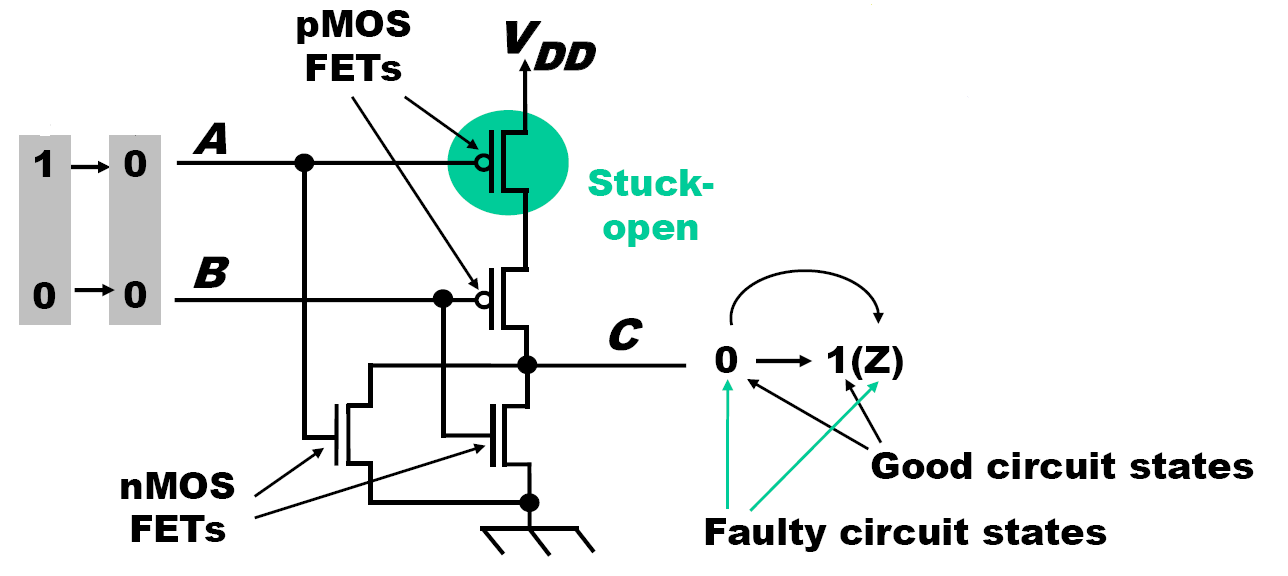
\includegraphics[scale=0.235]{img/stukopen.png}
\label{fig:stukopen}
}
\subfigure[stuk-short]{
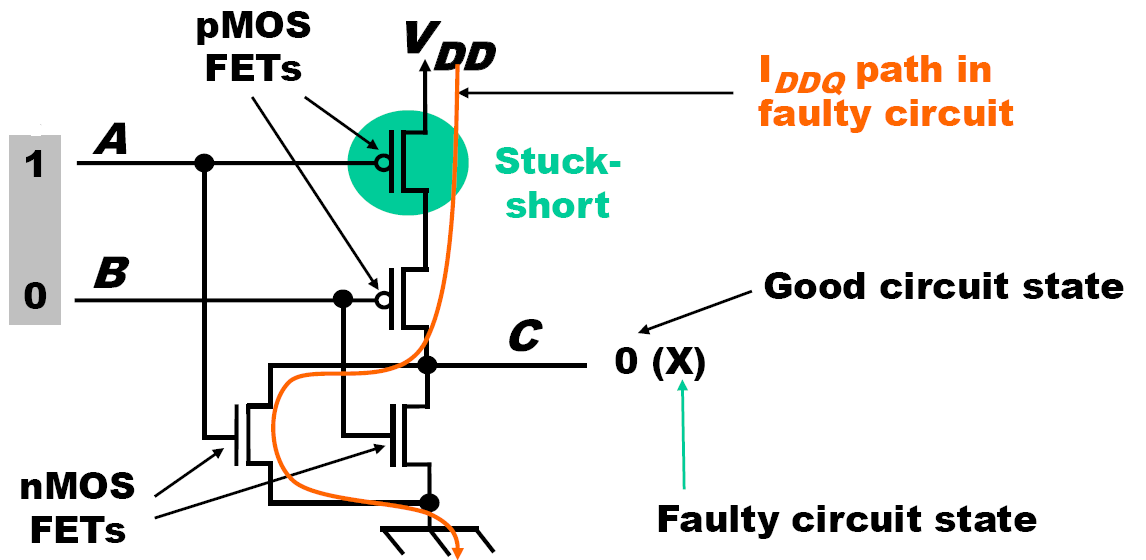
\includegraphics[scale=0.235]{img/stukshort.png}
\label{fig:stukshort}
}
\caption{Esempio di stuck-open e stuck-short}
\end{figure}
\subsection{Fault simulation}
Dopo aver capito che cos'è un modello di guasto passiamo ora a capire come sfruttarlo all'interno di una simulazione.
Per effettuare una simulazione si parte sempre da un circuito, nella maggior parte dei casi questo è espresso a livello logico, da una sequenza di vettori di test e da un modello di guasto; questo per determinare la copertura dei guasti individuati dall'insieme dei vettori di test, ma anche gli eventuali guasti non coperti per migliorare ed ottimizzare i collaudi post-produzione.
In alcuni casi la simulazione è utile anche per identificare quelle aree di test che risultano difficili da testare in modo che i progettisti possano valutare la possibilità di aggiungere della logica per aumentarne la testabilità; questo tipo di progettazione è anche chiamata \emph{Design for Test (DFT)}.
In \figurename\,\ref{fig:testschema} vediamo quali sono le diverse utilità della simulazione dei guasti sia in termini di copertura dei guasti (\emph{fault coverage}) sia in termini di ottimizzazione dei test (\emph{test compactor}).
\begin{figure}
\centering
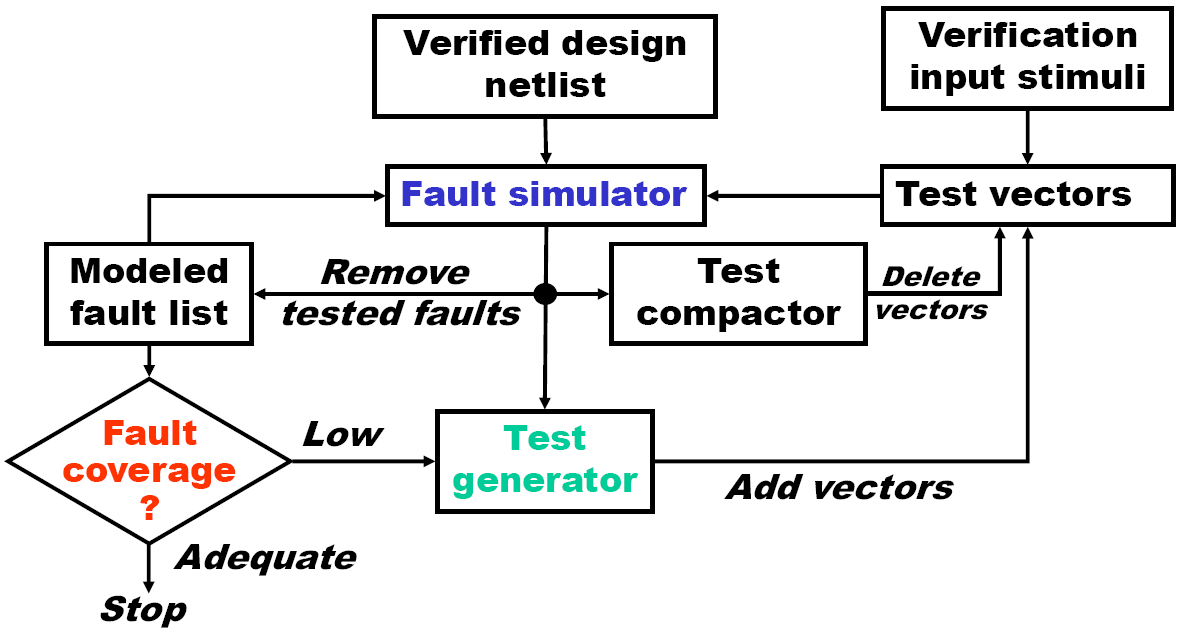
\includegraphics[scale=0.35]{img/testschema.png}
\caption{Diagramma che mostra il procedimento e l'utilità della \emph{fault simulator}}\label{fig:testschema}
\end{figure}
Un'altra funzionalità per cui la simulazione dei guasti è utilizzata è quella di \emph{timing} ovvero capire i tempi di transitorio che il circuito ha in presenza di guasti, in quanto potrebbe essere che il circuito ottenga un valore corretto ma che il tempo del transitorio sia maggiore di quello di clock e quindi non riuscirei ad analizzarlo. Questo tipo di simulazione è stata introdotta solamente negli ultimi anni quando le frequenze sono aumentate considerevolmente.\\
Gli algoritmi per la simulazione dei guasti sono diversi con diversi gradi di difficoltà, queste simulazioni sono:
\begin{itemize}
\item Seriale
\item Parallela
\item Deduttiva
\item Concorrente
\item e molti altri ancora
\end{itemize}
\subsubsection{Simulazione seriale}
Il primo tipo di simulazione che andiamo ad analizzare è quella che sfrutta un algoritmo di tipo \emph{seriale} in quanto è quello più semplice.\\
Si parte da una simulazione del circuito senza guasti in modo da registrare le uscite del circuito. A questo punto si effettua un'\emph{iniezione del guasto} ovvero si modifica il modello per far si che sia presente il guasto. A questo punto si riapplica il vettore di test al circuito e se la risposta differisce dal caso senza guasto sono in grado di affermare che il vettore di test analizzato identifica il guasto appena testato. Questa operazione viene ripetuta per tutti i guasti nella lista dei guasti, alla fine di tutta la simulazione posso determinare quali guasti sono coperti da quel vettore di test.\\
Per simulare un guasto durante una simulazione abbiamo detto che dobbiamo fare una \emph{iniezione di guasto} questa tecnica però può essere implementata in due modi, il primo è passare di volta in volta al simulatore un circuito diverso dove è stato introdotto il guasto oppure passare al simulatore un circuito simile a quello da testare ma dove nei punti di guasto sono stati inseriti dei \emph{multiplexer} e selezionare i punti di guasto tramite i valori di controllo del multiplexer.\\
Lo svantaggio principale di questa tecnica è che richiede un notevole numero di simulazioni e le computazioni risultano ripetitive. Per risolvere tale problema si può sfruttare un certo grado di parallelizzazione.
\subsubsection{Simulazione parallela}
Nella simulazione parallela si utilizza una caratteristica dei processori, ovvero la possibilità di eseguire un \texttt{AND} o un \texttt{OR} di un intera parola (32 o 64 bit) in un unico ciclo di clock. L'idea è quella di compattare più di un simulazione durante un'unica computazione, sfruttando tale tecnica si possono testare $w-1$ (è necessario simulare anche il circuito senza guasti) guasti in un unica simulazione. Un esempio di questa tecnica è mostrato in \figurename\,\ref{fig:simparallel} dove si fa l'esempio di un processore a 3 bit e si testano due guasti con un'unica simulazione.
\begin{figure}
\centering
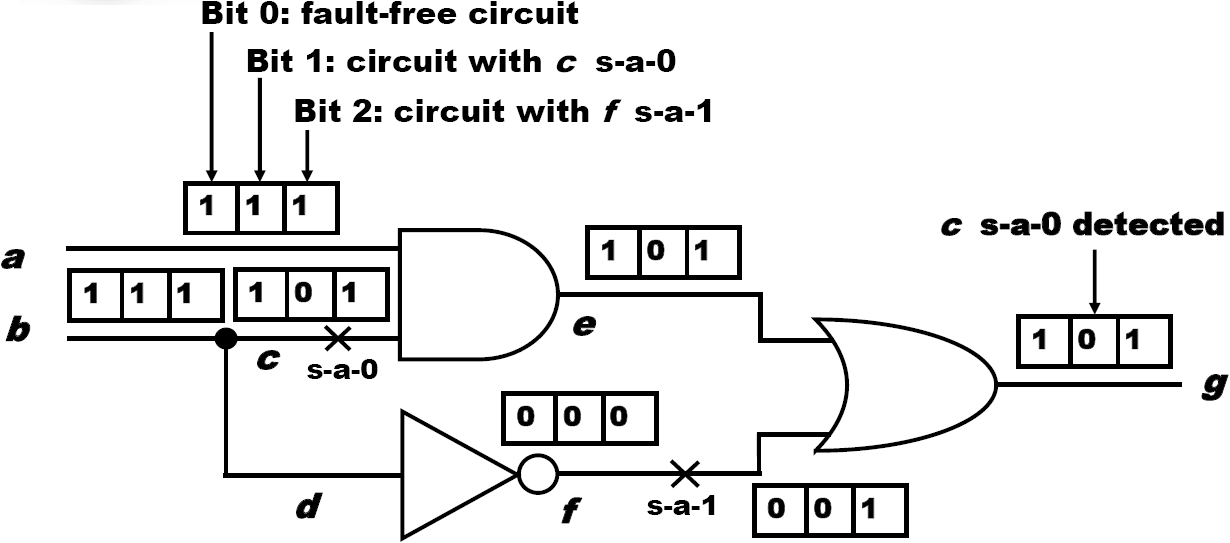
\includegraphics[scale=0.4]{img/simparallel.png}
\caption{Esempio di simulazione parallela con processore a 3 bit}\label{fig:simparallel}
\end{figure}
\subsubsection{S§imulazione deduttiva}
Nel caso di simulazione parallela si sfrutta la possibilità di parallelizzare i calcoli, tuttavia non si agisce sul fatto di riutilizzare le precedenti computazioni per quelle parti di circuito che non vengono toccate da guasti. La simulazione deduttiva, invece, sfrutta proprio questa caratteristica.
In questo caso si analizza il circuito con la presenza di tutti i guasti ma considerando un guasto alla volta. Tramite questa tecnica si riesce a calcolare l'insieme dei guasti individuabili tramite un determinato vettore di test utilizzando un'unica simulazione.\\
Il principio è quello di individuare tutti i possibili guasti di una determinata linea \emph{k} e inserirli in una lista $L_k$ e a questo punto applicare delle regole insiemistiche delle varie porte.
La lista dei guasti che si ottengono all'uscita è l'insieme dei guasti individuabili dal vettore di test utilizzato. 
Lo svantaggio di questa tecnica è che si applica solamente a circuiti logici booleani e non a quelli con \emph{flip-flop} o altri componenti.
In \figurename\,\ref{fig:deductivesim} vediamo un esempio di questa tecnica, all'uscita della porta \texttt{AND} abbiamo che l'insieme dei guasti rilevabili sono :
$$L_e=L_a\cup L_c \cup \{e_0\}=\{a_0,b_0,c_0,e_0\}$$
Questo perchè entrambe le linee di ingresso mostrano valori non dominanti nel caso invece della porta \texttt{OR} abbiamo che all'uscita i guasti individuati sono quelli dell'ingresso \emph{e} meno quelli dell'ingresso \emph{f} in quanto sull'ingresso \emph{f} è presente un valore non dominante.
\begin{figure}
\centering
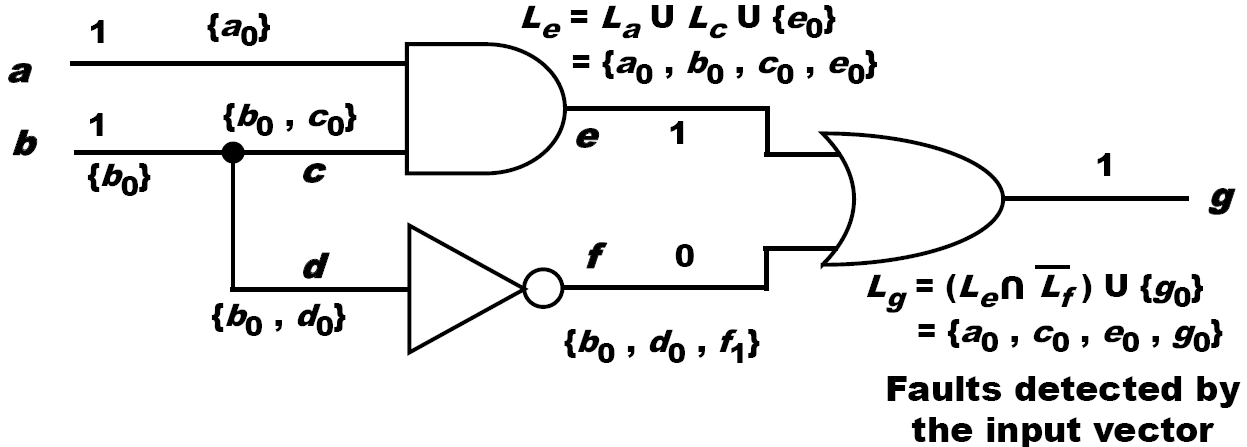
\includegraphics[scale=0.4]{img/deductivesim.png}
\caption{Esempio di simulazione deduttiva}\label{fig:deductivesim}
\end{figure}
\subsubsection{Simulazione concorrente}
La simulazione concorrente è molto simile a quella deduttiva, tuttavia in questo caso si parte da una simulazione priva di guasti e via via si iniettano i diversi guasti ricalcolando solamente le porte che subiscono una variazione dopo l'iniezione.
Questo sistema è molto più rapido dei precedenti, tuttavia il fatto di memorizzare lo stato delle porte che cambiano comporta un grande consumo di memoria.\\
In \figurename\,\ref{fig:concsim} vediamo un esempio di tale tecnica, si nota subito come l'ultima porta or debba tener conto di tutti i guast.
\begin{figure}
\centering
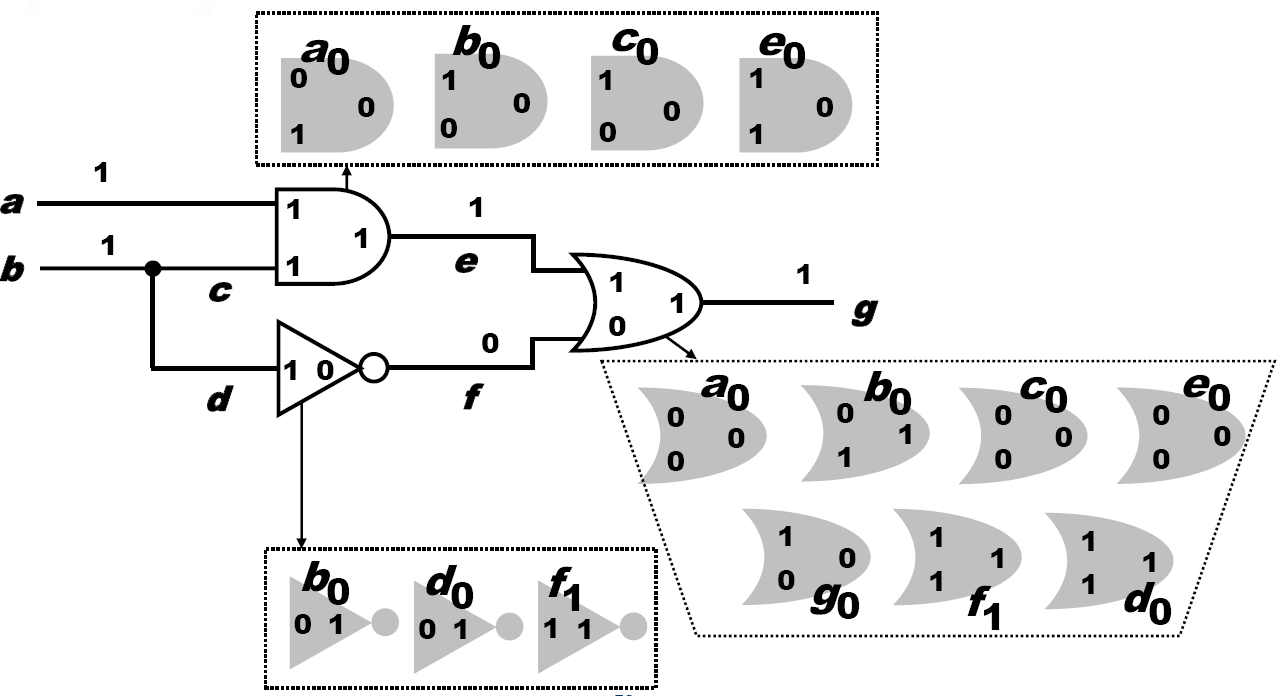
\includegraphics[scale=0.35]{img/concsim.png}
\caption{Esempio di simulazione concorrente}\label{fig:concsim}
\end{figure}
\subsubsection{Simulazione di vettori parallela}
Questo tipo di simulazione è molto simile a quella parallela ma in questo caso non si testano diversi guasti con lo stesso vettore bensì si testa un guasto diversi vettori di test. Questa tecnica è utile soltanto se il circuito è privo di memoria. In caso contrario tale tecnica è inapplicabile.
\subsubsection{Fault samplig}
In moti casi è impossibile testare tutti i guasti, tuttavia è possibile ottenere una buona copertura utilizzando il \emph{fault samplig}. Si tratta di scegliere un sottoinsieme casuale dei guasti ed effettuare la simulazione su questi guasti per calcolarne la copertura. La misura di copertura dei guasti su questo sottoinsieme ci da una misura sulla copertura totale dei guasti. Questo meccanismo permette di risparmiare molto tempo nelle simulazioni tuttavia può portare a non testare alcuni guasti.
\subsection{Generazione dei test nei circuiti combinatorio}
In questo paragrafo analizzeremo come creare i vettori di test che serviranno poi sia per la simulazione che per il collaudo del sistema.
In molti casi questi vettori sono generalmente gli stessi che il progettista usa per verificare la corretta funzionalità del sistema rispetto alle specifiche. Tuttavia in molti casi questi vettori non sono sufficienti e a volte necessari per valutare tutti i guasti. 
Prendiamo ad esempio il caso in \figurename\,\ref{fig:fulladder}, in questo caso tenendo conto solo della funzionalità e volendo testare completamente il circuito dovremmo utilizzare $2^{64}$ valori per il primo ingresso moltiplicati per $2^{64}$ valori per il secondo ingresso per l'ingresso di riporto per un totale di $2^{129}$ vettori di test. Nel caso in cui prendiamo in considerazione la struttura del circuito abbiamo che gli stuck-at per la parte di somma di un bit sono 10 mentre per la parte di riporto (non presente in \figurename) comprende 17 stuck-at questo significa per ogni singolo bit i guasti da testare sono 27 che moltiplicati per i 64 bit del sommatore fanno un totale di 1728 guasti; considerando il caso peggiore in cui sia necessario un vettore di test per ogni guasto abbiamo che sono necessari $1728 << 2^{129}$ vettori.\\
\begin{figure}
\centering
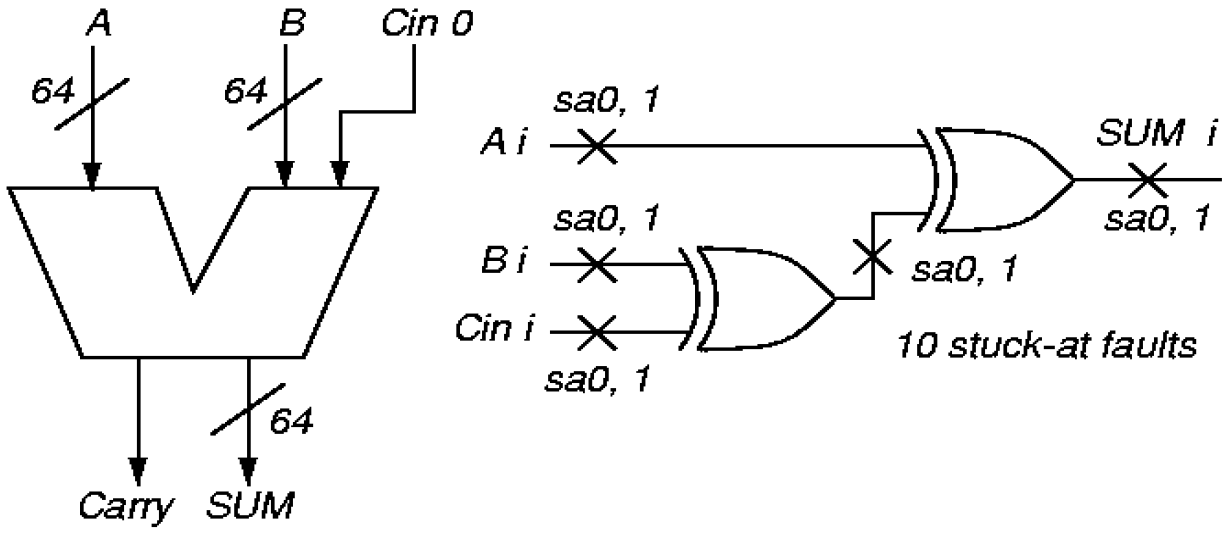
\includegraphics[scale=0.35]{img/fulladder.png}
\caption{Schema funzionale e strutturale di un full-adder con riporto}\label{fig:fulladder}
\end{figure}
Come abbiamo visto conoscere la struttura del circuito ci aiuta a ridurre i vettori di test, un altro fattore che aiuta nel ridurre la complessità delle simulazioni è l'utilizzo di un algoritmo per la generazione dei test che sia \emph{completo} ovvero per ogni guasto l'algoritmo è in grado di stabilire se questo è testabile o meno.\\
Un guasto \emph{non testabile} è un guasto che, pur essendo presente nel circuito, non influenza il comportamento di tale circuito ovvero non ne compromette la funzionalità, questo tipo di guasto è anche detto \emph{ridondante} ma solo nei circuiti combinatori e indica la presenza di hardware non necessario.\\
Per lo studio della generazione di test dobbiamo prima introdurre alcuni strumenti tra questi le algebre di \emph{Roth} e di \emph{Muth} espresse in \tablename\,\ref{tab:rothmuth}.
\begin{table}
\centering
\begin{tabular}{|c|c|c|cl|}
\hline
Symbol & Meaning & Good Machine & Failing Machine & \\
\hline
$D$ & $1/0$ & $1$ & $0$ & \\
$\overline{D}$ & $0/1$ & $0$ & $1$ & \\
$0$ & $0/0$ & $0$ & $0$ & Algebra di Roth\\
$1$ & $1/1$ & $1$ & $1$ & \\
$X$ & $X/X$ & $X$ & $X$ & \\
\hline
$G0$ & $0/X$ & $0$ & $X$ & \\
$G1$ & $1/X$ & $1$ & $X$ & Algebra di Muth\\
$F0$ & $X/0$ & $X$ & $0$ & \\
$F1$ & $X/1$ & $X$ & $1$ & \\
\hline
\end{tabular}
\caption{Notazioni delle algebre di Roth e di Muth}\label{tab:rothmuth}
\end{table}
Queste algebre permettono di simulare due macchine simultaneamente, il primo valore indica una macchina che funziona correttamente il secondo valore una macchina in errore, inoltre queste algebre sono di facile rappresentazione e risoluzione. Per trovare i vettori di test dobbiamo però fare delle premesse, il valore nel punto di guasto deve essere differente rispetto a quello dello stuck-at (deve essere presente una $D$ o una $\overline{D}$), il guasto deve essere propagato all'uscita (una $D$ o una $\overline{D}$ devono essere presenti sull'uscita).
Analizziamo ora alcuni dei principali algoritmi di generazione dei test.
\subsubsection{Algoritmo esaustivo}
Nel caso di un circuito con $n$ input si generano tutti i $2^n$ possibili vettori di test. Questo algoritmo è applicabile solo per un numero $n\leq 15$ di input altrimenti il numero di vettori risulta troppo grande. Tuttavia questo meccanismo può essere utilizzato su alcuni circuiti per effettuare dei test \emph{built-in} su una parte del circuito.
\subsubsection{Generazione casuale}
In questo caso i vettori di test sono generati casualmente. Questo meccanismo è utile soprattutto nel caso di circuiti aritmetici e fornisce dei risultati buoni con una copertura dei guasti che si aggira tra il 60\% e l'80\%. Questa tecnica è utilizzata anche in combinazione con altre tecniche per aumentare il grado di copertura.
\subsubsection{Path Sensitization}
La \emph{Path sensitization} è un algoritmo per l'individuazione dei vettori di test molto semplice e di facile applicazione. Esso si compone di tre passi:
\begin{enumerate}
\item \textbf{Fault Sensitization:} durante questo passo si innesta il guasto e a questo punto tramite l'algebra di Roth si inserisce una $D$ o una $\overline{D}$ nel punto di guasto (\figurename\,\ref{fig:pathsensi1})
\item \textbf{Fault Propagation:} durante questo passo si propaga il guasto verso l'uscita scegliendo uno o più percorsi come mostrato in \figurename\,\ref{fig:pathsensi2} e \figurename\,\ref{fig:pathsensi3}
\item \textbf{Line Justification:} a questo punto si impongono sulle linee restanti dei valori utili per completare il circuito. Nel caso in cui sia possibile (\figurename\,\ref{fig:pathsensi4}) ottengo il vettore di test, nel caso non sia possibile (\figurename\,\ref{fig:pathsensi2} e \ref{fig:pathsensi3}) scarto il circuito
\end{enumerate} 
\begin{figure}
\centering
\subfigure[Fault Sensitization]{
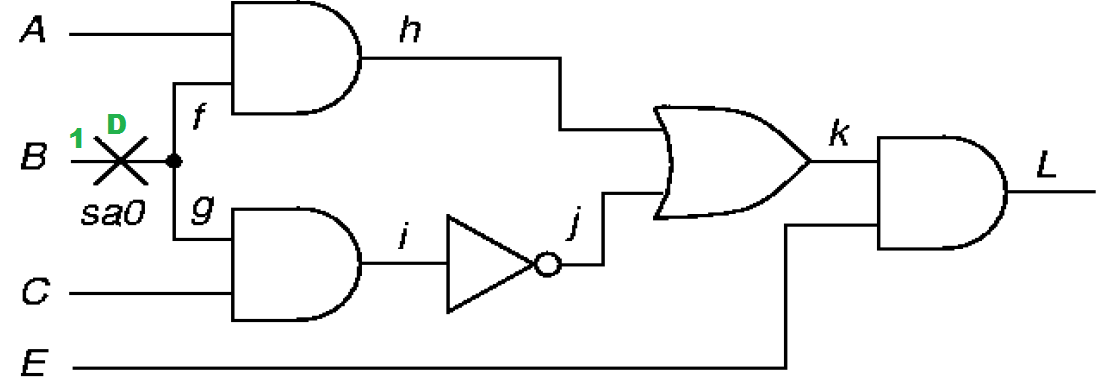
\includegraphics[scale=0.45]{img/pathsensi1.png}
\label{fig:pathsensi1}
}
\subfigure[Fault propagation sul percorso f-h-k-L]{
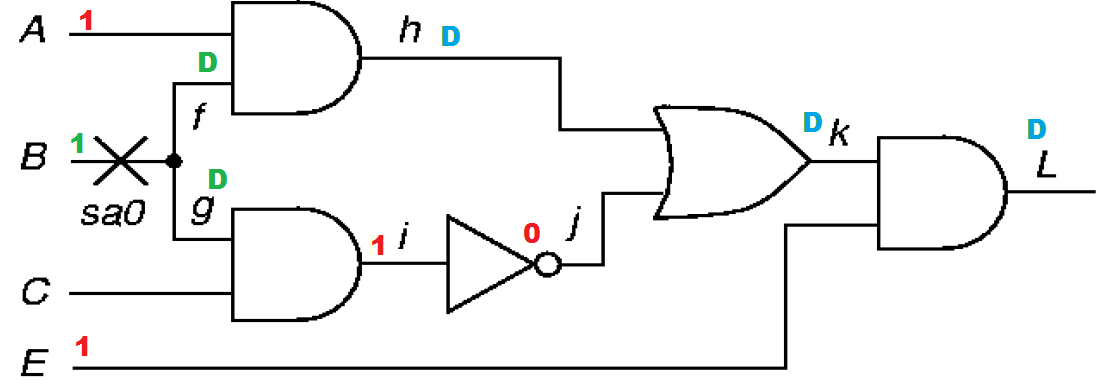
\includegraphics[scale=0.45]{img/pathsensi2.png}
\label{fig:pathsensi2}
}
\subfigure[Fault propagation parallela su f-h-k-L e g-i-j-k-L]{
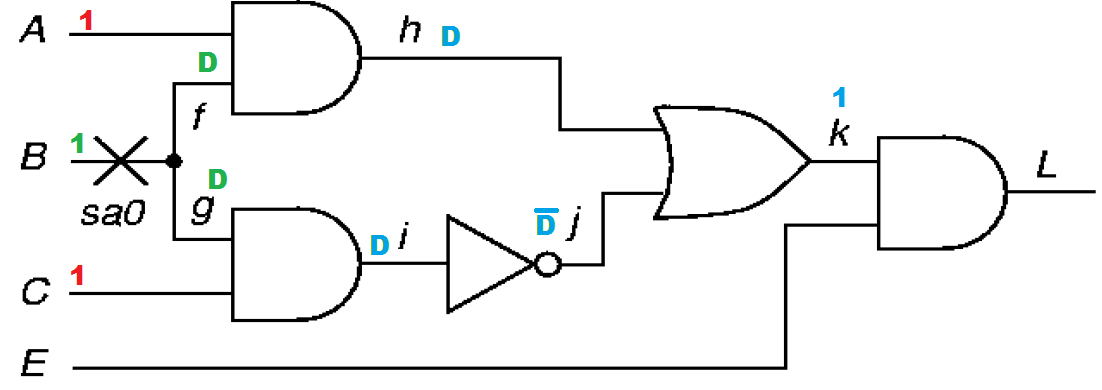
\includegraphics[scale=0.45]{img/pathsensi3.png}
\label{fig:pathsensi3}
}
\subfigure[Fault propagation su g-i-j-k-L]{
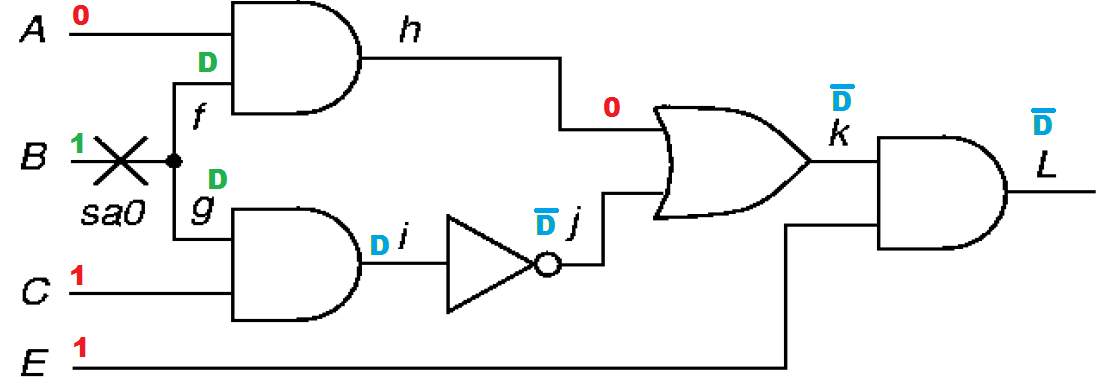
\includegraphics[scale=0.45]{img/pathsensi4.png}
\label{fig:pathsensi4}
}
\caption{Esempio di \emph{Path Sensitization}}
\end{figure}
Analizziamo più in dettaglio l'esempio, in \figurename\,\ref{fig:pathsensi1} vediamo come venga iniettato un guasto con stuck-at 0 ciò significa che l'ingresso \emph{B} deve essere inizializzato a \emph{1} altrimenti sarebbe impossibile individuare il guasto, inoltre secondo l'algebra di Roth un passio da $1\leftarrow 0$ va indicato da una $D$.\\
In \figurename\,\ref{fig:pathsensi2} il guasto viene propagato lungo il percorso \emph{f-h-k-L} tale propagazione è indicata in blu, dopo aver propagato il guasto fino all'uscita abbiamo cercato di andare a ritroso per riempire le linee rimaste vuote (numeri in rosso). In questo caso, per la porta \texttt{AND} con ingressi \emph{k} ed \emph{E} ad \emph{E} abbiamo assegnato il valore \emph{1}, alla porta \emph{AND} con ingressi \emph{A} e \emph{B} all'ingresso libero abbiamo assegnato il valore \emph{1}, infine, alla porta \texttt{OR} il cui ingresso \emph{j} era ancora libero abbiamo assegnato il valore \emph{0} e lo abbiamo propagato all'indietro fino ad avere in posizione \emph{i} il valore \emph{1}, tuttavia, questo valore è incompatibile con qualsiasi valore che avremmo potuto assegnare all'ingresso \emph{C}; questo porta a scartare il percorso.\\
In \figurename\,\ref{fig:pathsensi3} il guasto viene propagato parallelamente sia lungo il percorso \emph{f-h-k-L} sia lungo il percorso \emph{g-i-j-k-L}, in questo caso abbiamo che durante la propagazione del guasto il guasto scompare (valore \emph{1} in posizione \emph{k}) tale fenomeno è chiamato \emph{scomparsa della D-frontiera}.\\
Infine, in \figurename\,\ref{fig:pathsensi4} vediamo la propagazione del guasto lungo il percorso \emph{g-i-j-k-L} e vediamo come sia possibile sia portare il guasto fino all'uscita sia effettuare la \emph{Line Justification} ottenendo così il vettore di test per il guasto analizzato. Tale vettore corrisponde al vettore \emph{0-1-1-1} rispettivamente per gli ingressi \emph{A-B-C-E}.\\
Abbiamo visto come questo meccanismo sia molto semplice tuttavia non è molto efficiente, in caso di circuito con \emph{no\_pi} numero di ingressi primari e \emph{no\_ff} numero di flip-flop del circuito e volendo simulare \emph{n} porte logiche abbiamo che la la complessità è pari a :
$$O(n \times 2^{no\_pi} \ times 4^{no\_ff})$$
\newpage
\subsubsection{Algoritmo D}
Prima di iniziare a parlare di questo algoritmo dobbiamo introdurre alcuni concetti. Il primo concetto che introduciamo è quello del \emph{forward implication} la quale afferma che dati degli ingressi di porte logiche i quali sono etichettati in modo significativo è possibile determinare univocamente le uscite. Ad esempio per una porta \texttt{AND} la tabella della forward implication è mostrata in \figurename\,\ref{fig:forwardimp}.\\
\begin{figure}
\centering
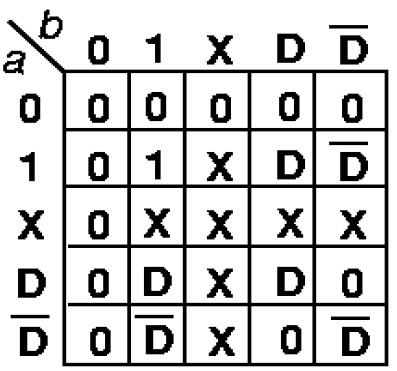
\includegraphics[scale=0.4]{img/forwardimp.png}
\caption{Forward implication table per una porta \texttt{AND}}\label{fig:forwardimp}
\end{figure}
Un'altra definizione è quella della \emph{backward implication} molto simile alla forward solo che in questo caso i valori noti sono quelli dell'output e a volte di uno degli ingressi e si riesce a risalire alle uscite, un esempio è mostrato in \figurename\,\ref{fig:backwardimp}.\\
\begin{figure}
\centering
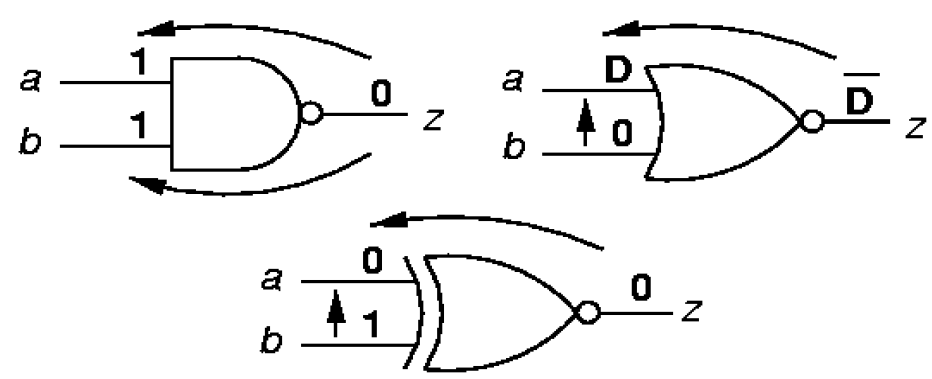
\includegraphics[scale=0.4]{img/backwardimp.png}
\caption{Esempi di backward implication}\label{fig:backwardimp}
\end{figure}
Durante la fase di decisione sui valori da assegnare agli ingressi può capitare che in alcuni punti possano essere possibili più scelte come ad esempio nel caso di una porta \texttt{AND} la cui uscita vale\emph{0}. Per tenere traccia di queste possibilità e delle decisioni prese si utilizza un \emph{implication stack} ovvero una tabella nella quale si tengono conto dei vari ingressi, del valore ad esso assegnati e se quel valore è l'unico possibile. Da questa tabella è possibile creare un \emph{albero delle decisioni} per tenere traccia di quali percorsi sono esplorabili, quali sono stati esplorati e quali no. Un esempio di albero delle decisioni è mostrato in \figurename\,\ref{fig:decisiontree}
\begin{figure}
\centering
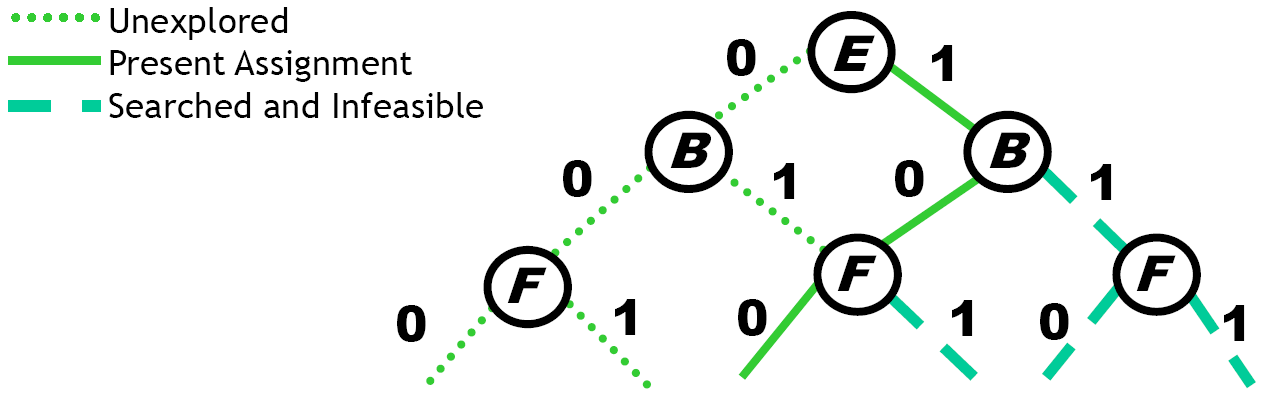
\includegraphics[scale=0.45]{img/decisiontree.png}
\caption{Esempio di albero delle decisioni}\label{fig:decisiontree}
\end{figure}
Questo tipo di algoritmo sfrutta il meccanismo del \emph{Branch and Bound} per trovare una soluzione, ad ogni livello dell'albero l'algoritmo selezione uno dei possibili input escludendo al tempo stesso porzioni dell'albero per restringere le decisioni possibili in quanto un'esplorazione completa dell'albero è impraticabile.\\
L'algoritmo \emph{D} è il primo algoritmo completo per la creazione di vettori di test, esso sfrutta oltre alle precedenti nozioni anche quella del \emph{D-Cube} e del \emph{D-Calculus}.
Il \emph{D-Cube} non è altro che il collassamento della tavola di verità del circuito utilizzando i valori dell'algebra di Roth.\\
L'algoritmo si compone di cinque passi
\begin{itemize}
\item Si numerano tutte le linee del circuito in modo incrementale dagli ingressi alle uscite.
\item Si seleziona una delle primitive 0che indicano il guasto dal \emph{D-Cube} 
\item Si effettua il D-drive ovvero la propagazione del guasto
\item Si verifica la consistenza
\item Si ripete l'operazione del D-drive
\end{itemize}
Un esempio è quello in \figurename\,\ref{fig:dalgoexe} mentre la \tablename\,\ref{tab:dcube} è la tabella D-Cube di copertura
\begin{table}
\centering
\begin{tabular}{|c|c|c|c|c|c|}
\hline
A & B & C & d & e & F \\
\hline
 1 & 1 &   & 1 &   &   \\
 0 &   &   & 0 &   &   \\
   & 0 &   & 0 &   &   \\
   & 1 & 1 &   & 0 &   \\
   & 0 &   &   & 1 &   \\
   &   & 0 &   & 1 &   \\
   &   &   &   & 1 & 0 \\
   &   &   & 1 &   & 0 \\
   &   &   & 0 & 0 & 1 \\
\hline
 $D$ & 1 &   & $D$ &   &   \\
 1 & $D$ &   & $D$ &   &   \\
 $D$ & $D$ &   & $D$ &   &   \\
   & $D$ & 1 &   & $\overline{D}$ &   \\
   & 1 & $D$ &   & $\overline{D}$ &   \\
   & $D$ & $D$ &   & $\overline{D}$ &   \\
   &   &   & $D$ & 0 & $\overline{D}$ \\
   &   &   & 0 & $D$ & $\overline{D}$ \\
   &   &   & $D$ & $D$ & $\overline{D}$ \\
\hline
\end{tabular}
\caption{Esempio di D-Cube di propagazione}\label{tab:dcube}
\end{table}
\begin{figure}
\centering
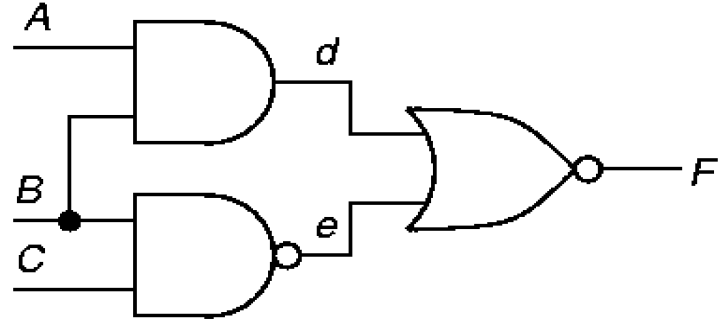
\includegraphics[scale=0.4]{img/dalgoexe.png}
\caption{Circuito di esempio per l'algoritmo D}\label{fig:dalgoexe}
\end{figure}
Volendo analizzare uno \emph{stuck-at 0} nel punto \emph{d} i passi sono tre e sono mostrati in \tablename\,\ref{tab:dalgoexe}.\\
\begin{table}
\centering
\begin{tabular}{|c|cccccc|c|}
\hline
\textbf{Step} & \textbf{A} & \textbf{B} & \textbf{C} & \textbf{d} & \textbf{e} & \textbf{F} & \textbf{Cube type}\\
\hline
1 & 1 & 1 &   & $D$ &   &   & Primitive D-cube of Failure \\
\hline
2 &   &   &   & $D$ & 0 & $\overline{D}$ & Propagazione D-Cube \\
\hline
3 &   & 1 & 1 &   & 0 &   & Backward implication \\
\hline
\end{tabular}
\caption{Passi per la generazione del test}\label{tab:dalgoexe}
\end{table}
Uno \emph{stuck-at 0} in \emph{d} significa che in quel punto abbiamo una $D$ utilizzando la backward implication otteniamo che sugli ingressi \emph{A} e \emph{B} abbiamo due 1. Sfruttando la seconda parte della \tablename\,\ref{tab:dcube} abbiamo che per un valore $D$ sulla linea \emph{d} abbiamo due possibilità (ultima e terzultima riga) prendiamo la prima delle due possibilità e questo ci dà il valore della linea \emph{e} ovvero 0. A questo punto per avere 0 sulla linea \emph{e} ed avendo già l'ingresso \emph{B} fissato al valore 1 l'unica soluzione possibile è che all'ingresso di \emph{C} abbiamo il valore 1.
Per un ulteriore esempio più esaustivo si rimanda alle slide del corso e al video dell'insegnante.
\newpage
\subsubsection{Algoritmo PODEM}
L'algoritmo PODEM introdotto nel 1981 introdusse il concetto che l'albero delle decisioni non doveva essere espanso a tutte le linee del circuito ma solamente agli ingressi primari, inoltre esso non andava ad analizzare tramite backward e forward implication se il vettore esisteva ma semplicemente controlla di volta in volta l'esistenza della \emph{D-Frontiera} ed infine utilizzava il \emph{backtracing}.\\
L'algoritmo di PODEM si svolge in 6 passi:
\begin{enumerate}
\item Si assegna un valore binario ad uno degli ingressi ancora libero.
\item Si determinano le implicazioni su tutti gli altri ingressi
\item Il vettore di test è stato generato? Se si \emph{fatto}.
\item Se è possibile assegnare valori ad altri ingressi tornare al punto 1
\item Esistono combinazioni di valori per gli ingressi non ancora testati? Se no il guasto è \emph{non testabile.}
\item Cercare una combinazione di valori per gli ingressi tramite obiettivi e backtrace.
\end{enumerate}
Per un esempio completo si rimanda alle slide del corso.
\subsection{Generazione dei test nei circuiti sequenziali}
Passiamo ora alla generazione dei test per circuiti sequenziali. Nei circuiti sequenziali sono presenti degli elementi di memoria il cui valore non è noto e perciò è necessario introdurre più vettori di test in sequenza che permettano di portare questi elementi in uno stato cososciuto e successivamente testare i guasti. Un esempio di questa tecnica è mostrato in \figurename\,\ref{fig:seqexemp} dove vediamo che dopo aver inserito agli ingressi il vettore \emph{1-1} non riusciamo ad individuare il valore dell'uscita ma possiamo inizializzare il flip-flop ad un valore noto. A questo punto è possibile applicare un secondo vettore di test per testare il guasto.
\begin{figure}
\centering
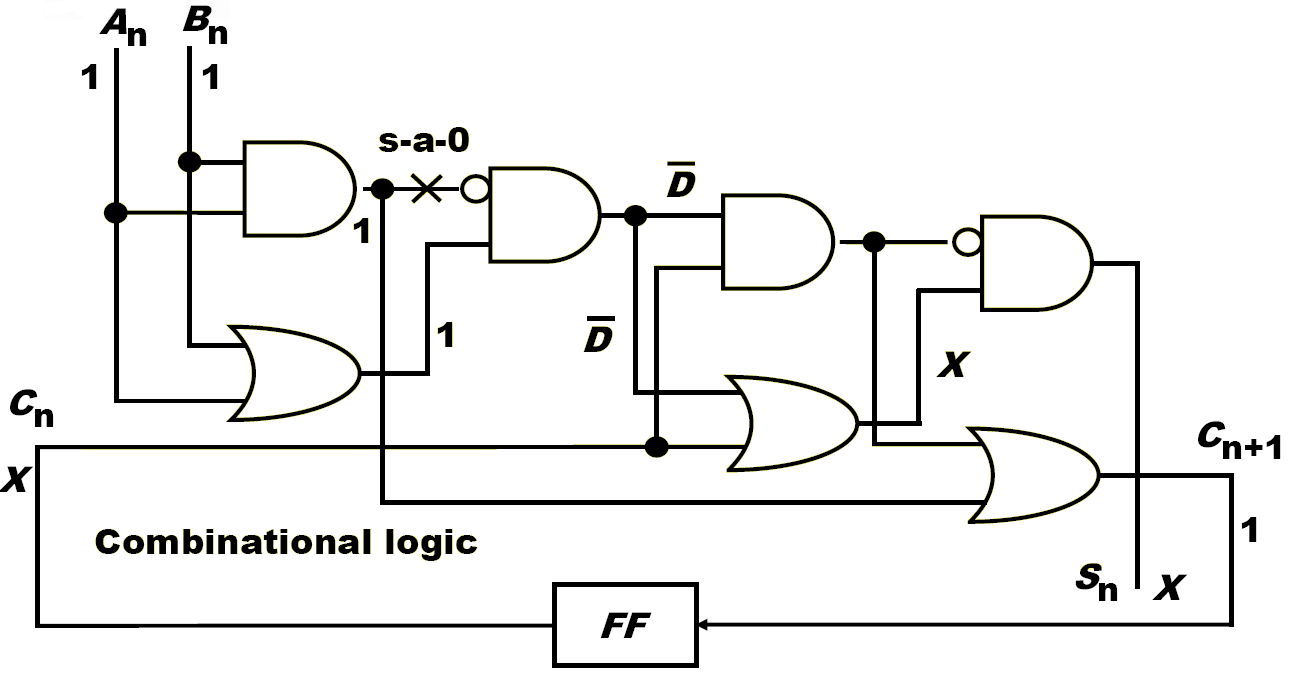
\includegraphics[scale=0.4]{img/seqexemp.png}
\caption{Esempio di circuito sequenziale}\label{fig:seqexemp}
\end{figure}
Per effettuare il test dei circuiti sequenziali come abbiamo detto è necessario applicare più vettori, ma per farlo dobbiamo applicare la \emph{time-frame expansion} che in pratica non fa altro che replicare \emph{n-volte} il circuito da testare (dove \emph{n} il numero di vettori di test) inserisce il guasto in ogni circuito ed infine genera i vettori di test utilizzando sia l'algebra di Roth che quella di Muth. Questo meccanismo permette di esplicitare il tempo tuttavia non si riesce a sapere a priori il numero di replicazioni necessarie.\\
Il meccanismo di risoluzione è molto simile ai precedenti:
\begin{itemize}
\item Si selezione un uscita sulla quale esporre il guasto.
\item Si posiziona il valore logico, 1/0 o 0/1 in base al tipo di guasto e al numero di inversioni.
\item Si giustificano le linee partendo dalle uscite e andando a ritroso verso gli ingressi.
\item Se non è possibile effettuare la giustificazione si seleziona una nuova uscita tramite la derivabilità.
\item Se tale tecnica fallisce per tutte le uscite raggiungibili allora il guasto è non testabile.
\item Se i valori 1/0 o 0/1 non sono giustificabili ma i valori 1/X o 0/X lo sono allora il guasto diventa \emph{potentially detectable}.
\end{itemize}
\begin{figure}
\centering
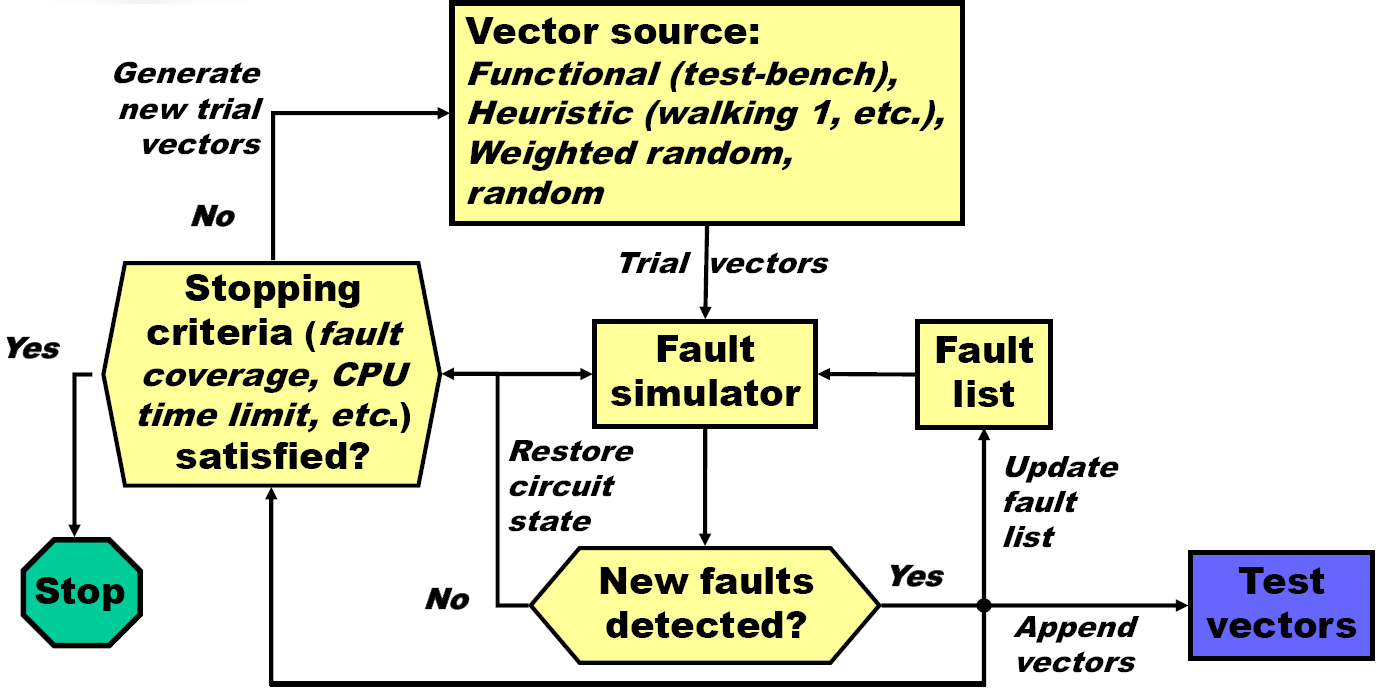
\includegraphics[scale=0.4]{img/simumeth.png}
\caption{Generazione dei vettori di test tramite simulazione}\label{fig:simumeth}
\end{figure}
Possiamo fare una distinzione tra i circuiti sequenziali, possiamo avere circuiti \emph{cycle-free} ovvero senza cicli nei quali non vi è alcun feedback tra i diversi flip-flop, in questo caso la generazione dei vettori è molto più semplice e richiede al massimo un espansione pari a $1+dseq$ dove \emph{dseq} è il grado di dipendenza dei \emph{ff}. Nel caso di circuiti con \emph{cicli} le cose si complicano ed è necessaria un espansione di $9^{N\_ff}$ dove \emph{N\_ff} è il numero di flip flop.\\
Analizziamo ora i diversi algoritmi per la generazione dei test nei circuiti sequenziali, questi algoritmi non sono algoritmi esatti come quelli utilizzati per i circuiti combinatori ma sfruttano la simulazione per trovare dei risultati. L'utilizzo della simulazione è dovuto al fatto che le sequenze da inizializzare sono molto lunghe ed è impossibile utilizzare un albero delle decisioni, inoltre i modelli dei circuiti sono limitati e l'espansione porta a raggiungere tali limiti molto in fretta; infine problemi di complessità e di corsa alle risorse rende il metodo \emph{time-frame} inutilizzabile.\\
I metodi basati sulla simulazione invece sfruttano le già collaudate tecnologie di simulazione dei guasti inoltre i modelli sono già stati creati e verificati, le metodologie che si possono utilizzare sono diverse.
Un diagramma che riassume tale metodologia è mostrato in \figurename\,\ref{fig:simumeth}.
\subsubsection{Metodo Contest}
In questo tipo di simulazione vengono testati più vettori concorrentemente e vengono via via migliorati tramite l'utilizzo di una \emph{funzione di costo}. Tale metodo si suddivide in tre fasi:
\begin{itemize}
\item Una fase \emph{iniziale} nella quale non si tiene conto di nessun guasto e la funzione di costo viene calcolata con il circuito allo stato originale
\item Fase \emph{concorrente} vengono introdotti tutti i guasti, la funzione di costo viene calcolata in modo concorrente su più simulazioni.
\item Fase \emph{singolo guasto}, in questa fase si analizza un solo guasto alla volta utilizzando i valori della simulazione.
\end{itemize}
La funzione di costo definisce l'obiettivo che si vuole perseguire come l'inizializzazione dei vettori o la testabilità di un guasto, la funzione di costo si annulla quando i vettori trovati rispettano l'obiettivo.
Un esempio molto banale del meccanismo è mostrato in \figurename\,\ref{fig:contest}.\\
\begin{figure}
\centering
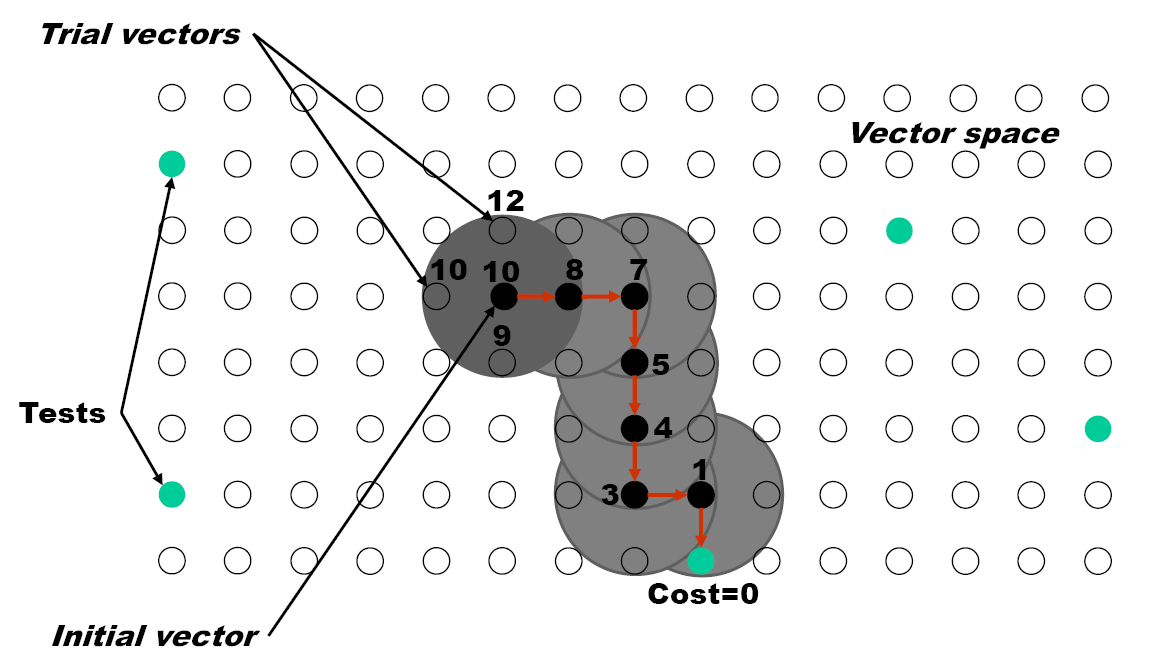
\includegraphics[scale=0.4]{img/contest.png}
\caption{Esempio di ricerca tramite funzione obiettivo}\label{fig:contest}
\end{figure}
\subsubsection{Algoritmo genetico}
L'algoritmo genetico afferma che una \emph{popolazione} migliora con ogni \emph{generazione}. 
Nel caso di generazione di vettori di test la popolazione è per l'appunto un insieme di vettori, il fattore di miglioramento è una qualità misurabile come una funzione di costo. Al funzione di rigenerazione invece viene trovata in modo euristico considerando i vettori più \emph{promettenti} e trasformandoli.
\subsubsection{Metodo spettrale}
Il \emph{metodo spettrale} si può considerare un evoluzione di quello genetico. Si parte da un insieme casuale di vettori di test si effettua un compattamento eliminando quelli non necessari o quelli ridondanti, dopo di che si simulano i diversi vettori. Lo schema di tale meccanismo è mostrato in \figurename\,\ref{fig:spectralmet}.
\begin{figure}
\centering
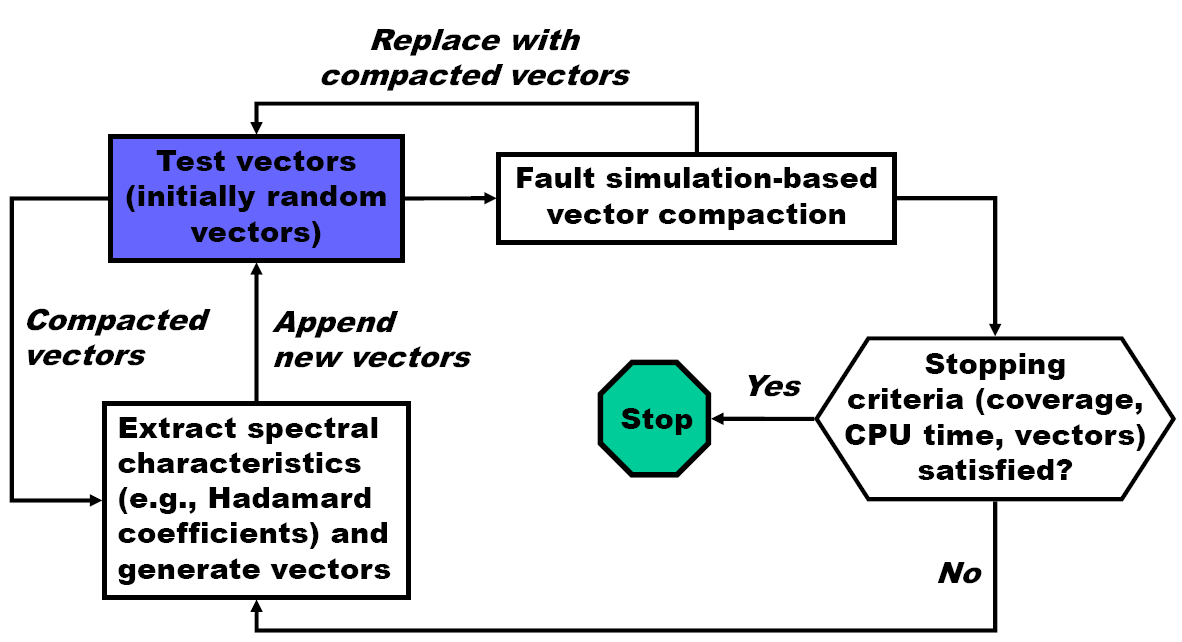
\includegraphics[scale=0.4]{img/spectralmeth.png}
\caption{Schema di riepilogazione del meccanismo spettrale}\label{fig:spectralmet}
\end{figure}